Een certificaat voor een webserver bevat:
\begin{itemize}
\item De public key van de server
\item De domeinnaam waarvoor het certificaat geldig is
\item De geldigheidsduur
\item De handtekening (signature) van de CA
\end{itemize}

Een voorbeeld van een signature is te zien in figuur \ref{img:cert:letsencrypt}.

\begin{figure}[h]
\centering
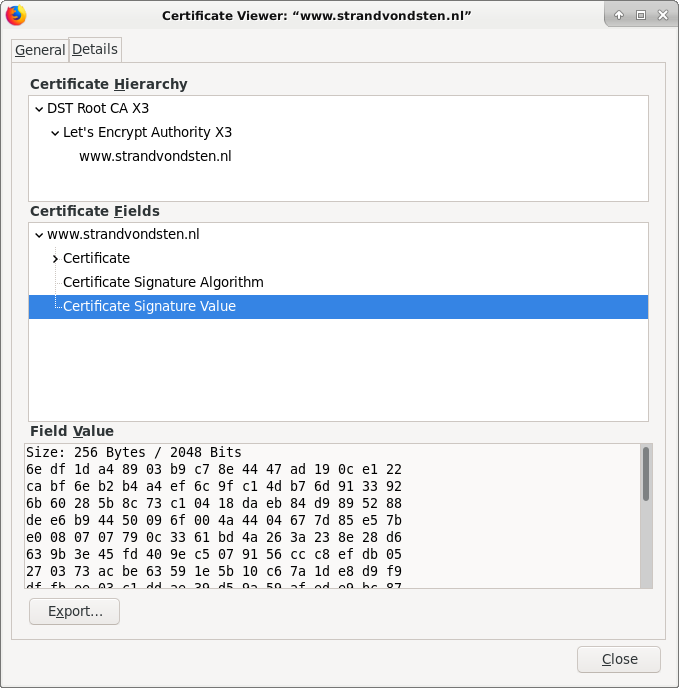
\includegraphics[width=0.8\textwidth]{Certificaat_LetsEncrypt.png}
\caption{Let's Encrypt certificaat}
\label{img:cert:letsencrypt}
\end{figure}

Een webserver heeft zijn eigen private key en het certificaat ge\"installeerd staan, en eventueel nog alle tussen liggende certificaten tussen het eigen certificaat en dat van de Certificate Authority.

Zodra een webbrowser contact maakt met een server en om een beveiligde verbinding vraagt stuurt de webserver zijn certificaat op naar browser. De browser controleert het certificaat door controle van het domeinnaam waarvoor het cerificaat geldig is, de geldigheidsduur van het certificaat en hij controleert de handtekening van de CA met die welke hij kent uit zijn database. Elke browser moet dus een lijst met bekende CA's hebben om deze controle te kunnen doen. Als het certificaat in orde wordt bevonden kan de public key uit het certificaat gebruikt worden om een encrypt bericht aan de server te sturen die dat bericht can decrypten met zijn private key.
